\section{Set-Up}
For the study of the QHE a two-dimensional or quasi two-dimensional system is needed.
In this experiment a quantum well is created by confining electrons in a thin layer of HgTe between
two layers of HgCdTe. Because of the smaller bandgap of HgTe compared to HgCdTe a quantum well is formed. 
At low temperatures (liquid helium), all electrons are located in the lowest energy level of the 
two dimensional quantum well. This creates a confinement in the layer stacking direction.
Inside the quantum film of HgTe, the electrons form a two-dimensional electron gas (2DEG) with high mobility.
All measurements are done in a variable temperature insert (VTI), which allowes to cool the sample down to a
range between roughly $4.2\,\text{K}$ and $1.5\,\text{K}$. The sample is designed in a common Hall bar geometry,
with in total $8$ contacts on the edges with a additional pair for the Gate voltage (see fig.\,\ref{fig:HallBar})
\begin{figure}[h]
    \centering
    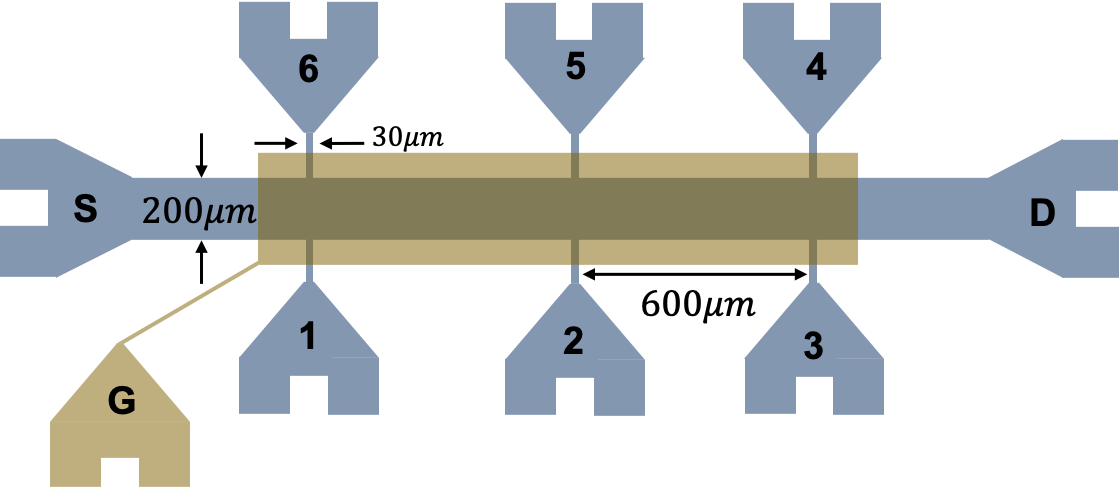
\includegraphics[width=0.45\textwidth]{../Images/HallBar.png}
    \caption{Schematic of the Hall bar geometry. The contacts are labeled with "S" for source, "D" for drain,
    "G" for gate. Contacts $4$ and $6$ are used for the measurement of the longitudina resistance 
    and contacts $3$ and $4$ are used for the measurement of the transversal resistance.}
    \label{fig:HallBar}
\end{figure}
An AC voltage is applied between source and drain to control the longitudinal current $I$
flowing through the sample. $I$ can be measured via the voltage drop $U_\text{I}$ over a known resistor $(R_\text{S}=4.982\pm0.0005)\,\text{k}\Omega$, 
which is connected in series to the source contact. $U_\text{I}$ is measured with a Lock In amplifier 
\emph{Stanford Research Systems SR510}. Contacts $3$ and $4$ are used to measure the hall voltage $U_\text{Hall}$, which
is measured with a second Lock In amplifier of the same type. Contacts $4$ and $6$ are used to measure
the longitudinal Voltage $U_\text{xx}$, which is measured with a third Lock In amplifier \emph{Stanford Research Systems SR530}.
For observation of the hall effect, a magnetic field $B$ is applied perpendicular to the plane of the sample.
The magnetic field is generated by a superconducting NbTi solenoid, which is cooled with liquid helium and can
be precisely controlled by the current flowing through the magnet. The flux density $B$ is read out as a voltage
$U_\text{B}$ with $U_\text{B}=10\,\text{V}$ corresponding to $